\subsection{Vorbereitung der Daten und deskriptive Analysen}
Die erhobenen Daten wurden mittels SPSS Version 25 für Mac OS X aufbereitet. Die Stichprobendaten wurden direkt aus der Enterprise Feedback Suite \cite{Questback2018} mittels Datenexport für SPSS exportiert. Allfällige Fehlerquellen wurden bei der Datenbereinigung korrigiert. Dies wurde durch die Umfragesoftware erleichtert, indem nur abgeschlossene Datensätze exportiert wurden und eine erste Werteprüfung bereits bei der Eingabe erfolgte (z.B.: es wurden nur Zahlen bei der Eingabe des Jahrgangs zugelassen). Fehlende Werte wurden bereits von der Umfragesoftware gesetzt und konnten innerhalb von SPSS mit einem Wertelabel versehen werden. Für die Berechnung der Mediennutzung, der Bindung, des Stressniveaus und des subjektiven Wohlbefindens wurden zusätzliche Variablen in SPSS erstellt und anhand der generierten Daten berechnet (für die Formel der Berechnung siehe Kapitel \titleref{sec:Design}).

\subsubsection{Medien und Mediennutzung}
Im Rahmen der Umfrage wurde die Mediennutzung während der Kindsbetreuung erhoben. Dabei wurde unterschieden zwischen \textit{privat genutzt}, \textit{geschäftlich genutzt}, \textit{privat \& geschäftlich genutzt} und \textit{nicht genutzt}. In Folge der Übersichtlichkeit wurde in Abbildung \ref{fig:Mediennutzung} die Ausprägung auf \textit{genutzt} und \textit{nicht genutzt} zusammengefasst, wobei die geschäftliche Nutzung in die private Nutzung miteinbezogen wurde (für die detaillierte Unterteilung anhand geschäftlich und privat bitte Anhang \ref{app:Mediennutzung} Abbildung \ref{fig:AppMediennutzung} konsultieren).

Demzufolge gaben 97.2\% der Befragten an, das Smartphone während der Betreuung zu benutzen gegenüber 2.8\%, die das Smartphone während der Betreuung nicht benutzten. Beim Medium TV gaben 31.7\% gegenüber 68.3\% an, diesen zu nutzen. Den Computer (Laptop- oder Desktopcomputer) nutzten 42.4\% und das Tablet nutzten 19.7\% während der Betreuung. Den Radio (Stereoanlage, CD Player) nutzten 62.8\%, Printmedien (Buch, Zeitung, Heft, Comic) 68.8\% und die Foto- oder Videokamera nutzten 55\%. Die Spielkonsole wurde von 4.1\% der Befragten während der Betreuung genutzt und der MP3 Player von 8.3\%.

% Figure
\begin{figure}[htp]
\caption{Medien \& Mediennutzung}\label{fig:Mediennutzung}
\centering
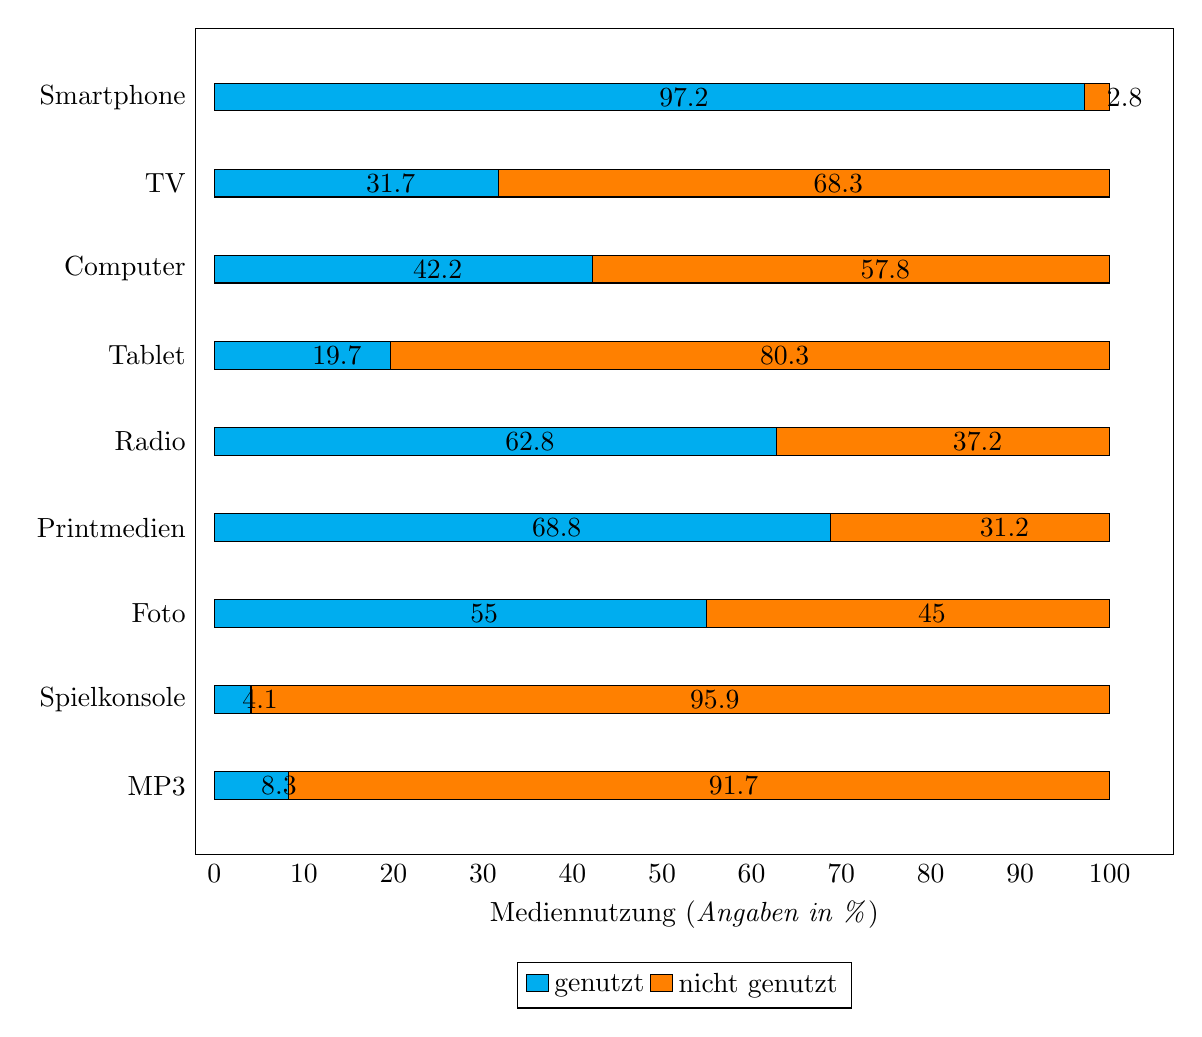
\begin{tikzpicture}[scale=1, auto,swap]
  \begin{axis}[
    xbar stacked,
    %y axis line style = { opacity = 0 },
    %axis x line       = none,
    tickwidth         = 0pt,
    xmin              = 0,
    xmax              = 105,
    enlarge y limits  = 0.1,
    enlarge x limits  = 0.02,
    %/legend pos=south east,
    legend style={at={(0.5,-0.13)}, anchor = north},
    legend columns     = -1,
    %reverse legend,
    ytick             = data,
    xlabel            = {Mediennutzung (\textit{Angaben in \%})},
    %height            = 20cm,
    width             = 14cm,
    symbolic y coords = {MP3, Spielkonsole, Foto, Printmedien, Radio, Tablet, Computer, TV, Smartphone},
    nodes near coords,
    nodes near coords align={horizontal},
  ]
  %benutzt
  \addplot[draw=black,fill=cyan] coordinates { (97.2,Smartphone)(31.7,TV)(42.2,Computer)(19.7,Tablet)(62.8,Radio)(68.8,Printmedien)(55,Foto)(4.1,Spielkonsole)(8.3,MP3)};
  \addlegendentry{genutzt~}
  %nicht genutzt
  \addplot[draw=black,fill=orange] coordinates { (2.8,Smartphone)(68.3,TV)(57.8,Computer)(80.3,Tablet)(37.2,Radio)(31.2,Printmedien)(45,Foto)(95.9,Spielkonsole)(91.7,MP3)};
  \addlegendentry{nicht genutzt}
  
  \end{axis}
\end{tikzpicture}
\end{figure}

Die Medientätigkeit in Minuten wurde anhand der letzten Betreuung des Kindes erfasst. Dabei wurde unterschieden, ob das Kind wach war oder geschlafen hat. Alle verwendeten Medien summiert ergab den Mittelwert der Medientätigkeit. Dieser belief sich während das Kind wach war auf $M$=93.1 Minuten ($SD$=103.6, $Min$=0, $Max$=613) und $M$=108.6 Minuten, währendem das Kind geschlafen hat ($SD$=105.3, $Min$=0, $Max$=495). Im Total waren die Teilnehmer im Schnitt $M$=202.1 Minuten mit Medien beschäftigt, währendem sie ihr Kind betreuten ($SD$=174.9, $Min$=3, $Max$=840) (Siehe dazu auch Tabelle \ref{table:Medientätigkeit}).

%Table
\begin{table}%[htbp]
\begin{tabular}{m{8em} m{4em}  m{4em}  m{5em} m{4em}} 
  \hline
  & $M$ & $SD$ & Min - Max & Schiefe\\
  \hline
  $MNS_{Wach}$* & 93.08 & 103.61 & 0 - 613 & 2.26\\
  $MNS_{Schlafend}$** & 108.63 & 105.32 & 0 - 495 & 1.56\\
  $MNS_{Total}$*** & 202.10 & 174.86 & 3 - 840 & 1.44 \\
  \hline
  \multicolumn{5}{l}{\textit{Anmerkung. *$N$=208, **$N$=205, ***$N$=204, Angaben in Minuten.}}\\
  &&&&\\
\end{tabular}
\caption{Medientätigkeit während der Betreuung}
\label{table:Medientätigkeit}
\end{table}

Auf die einzelnen Medien verteilt bedeutet dies, dass die Probanden im Schnitt $M$=5.2 Minuten telefoniert haben, während dem das Kind wach war und $M$=7.2 Minuten währendem das Kind geschlafen hat (siehe dazu Abbildung \ref{fig:Medientätigkeit}). Im Schnitt haben die Teilnehmer $M$=10 Minuten mit Textnachrichten verbracht (lesen und schreiben) während das Kind war wach und $M$=13.8 Minuten währendem das Kind geschlafen hat. Für das bearbeiten und Lesen von Emails setzten die Teilnehmer $M_{w}$=1.7 Minuten (Kind war wach) und $M_{s}$=7 Minuten ein (Kind hat geschlafen). Beim Lesen und Anschauen von Printemedien ((Bilder-)Bücher, Magazinen, Zeitungen, Comics, etc.) setzten die Eltern $M_{w}$=5.3 und $M_{s}$=12.5 Minuten ein. Im Internet verbrachten sie $M_{w}$=5.9 und $M_{s}$=19.7 Minuten mit Surfen und Informationen suchen. Musik hörten die Eltern während der Betreuung $M_{w}$=18.6 und $M_{s}$=8.3 Minuten. Sie schauten im Schnitt $M_{w}$=5.4 und $M_{s}$=25.1 Minuten Fernseh oder Videos (TV-Sender, Netflix, DVD, etc.). Der Radio lief während $M_{w}$=34.3 und $M_{s}$=12.9 Minuten. Fotos oder Videos wurden während $M_{w}$=5.1 und $M_{s}$=0.9 Minuten gemacht. Video-Games (Smartphone, Computer, Konsole, etc.) wurden während $M_{w}$=.2 und $M_{s}$=1.5 Minuten gespielt. Hörspiele und Hörbücher wurden während $M_{w}$=1.5 und $M_{s}$=2.1 Minuten gehört. Für eine komplette Auflistung der Mittelwerte nach der Unterteilung ob das Kind geschlafen hat oder wach war, inklusiver Angabe des totalen Mittelwerts bitte Tabelle \ref{fig:AppMedientätigkeit} im Anhang \ref{app:Medientätigkeit} konsultieren.

\begin{figure}%[htp]
\caption{Mittelwerte der Medientätigkeiten während der Betreuung}\label{fig:Medientätigkeit}
%\centering
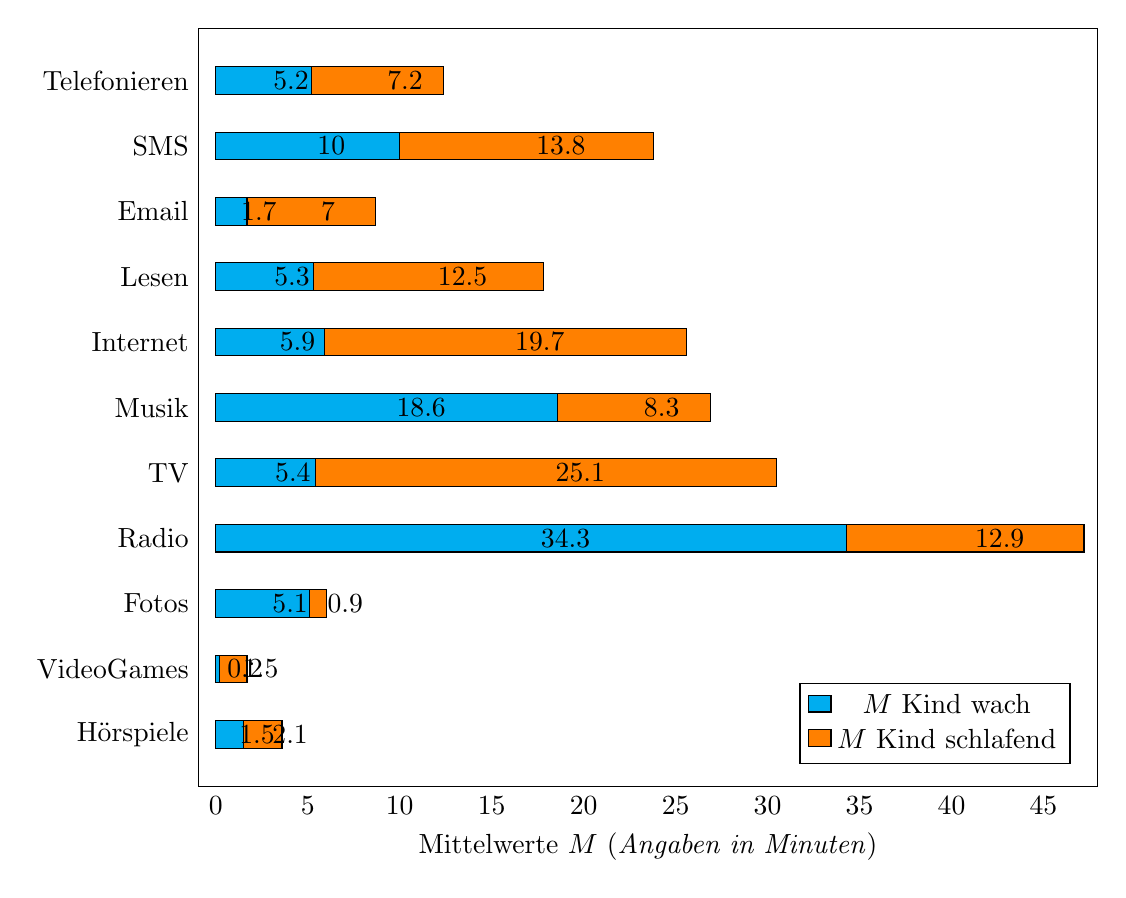
\begin{tikzpicture}[scale=1]
  \begin{axis}[
    xbar stacked,
    %y axis line style = { opacity = 0 },
    %axis x line       = none,
    tickwidth         = 0pt,
    xmin              = 0,
    xmax              = 47,
    enlarge y limits  = 0.08,
    enlarge x limits  = 0.02,
    legend pos=south east,
    ytick             = data,
    xlabel            = {Mittelwerte $M$ (\textit{Angaben in Minuten})},
    %height            = 20cm,
    width             = 13cm,
    symbolic y coords = {Hörspiele, VideoGames, Fotos, Radio, TV, Musik, Internet, Lesen, Email, SMS, Telefonieren},
    nodes near coords,
    nodes near coords align={horizontal},
  ]
  %wach
  \addplot[draw=black,fill=cyan] coordinates { (5.2,Telefonieren)(10,SMS)(1.7,Email)(5.3,Lesen)(5.9,Internet)(18.6,Musik)(5.4,TV)(34.3,Radio)(5.1,Fotos)(.2,VideoGames)(1.5,Hörspiele)};
  
  %schlafend
  \addplot[draw=black,fill=orange] coordinates { (7.2,Telefonieren)(13.8,SMS)(7,Email)(12.5,Lesen)(19.7,Internet)(8.3,Musik)(25.1,TV)(12.9,Radio)(0.9,Fotos)(1.5,VideoGames)(2.1,Hörspiele)};
  
  \legend{\text{$M$ Kind wach}, \text{$M$ Kind schlafend}}
  \end{axis}
\end{tikzpicture}
\end{figure}

Neben der Mediennutzung und der Medientätigkeit wurde die Anzahl Geräte im Haushalt erfragt (siehe dazu Tabelle \ref{fig:AppGeräteHaushalt} im Anhang \ref{app:Mediengeräte}). Dabei gaben 83.9\% der Teilnehmer an, 2 Smartphones im Haushalt zu besitzen. 70.2\% gaben an, ein TV-Gerät zu besitzen. 45\% der Befragten besitzen 2 Computer (Desktop oder Laptop), 45.9\% ein Tablet und 48.2\% einen Radio (Stereoanlage, CD-Player). 51.4\% gaben an, kein Abo einer Tageszeitung oder eines Magazins aboniert zu haben. 45.9\% gaben an, einen Fotoapparat oder Videokamera zu besitzen. 61\% besitzen keine Spielkonsole und 67\% keinen MP3 Player.

In der letzten Frage wurden von den Teilnehmern die drei Medien erhoben, auf die sie während der Betreuung ihres Kindes am wenigsten verzichten konnten. 85.3\% gaben an, nicht auf das Smartphone verzichten zu können, gefolgt vom Radio (Stereonalage, CD-Player) von 33.9\% und 25.2\% Foto- und Videokamera (siehe Tabelle \ref{fig:AppMedienverzicht} im Anhang \ref{app:Medienverzicht}). Weiter gaben die Teilnehmer an, dass 11.9\% von ihnen nicht auf den Fernseher, 9.6\% nicht auf das Abo einer Tageszeitung oder Zeitschrift, 8.3\% nicht auf den Computer (Laptop oder Desktop), 2.8\% nicht auf den MP3-Player, 2.3\% nicht auf das Tablet und .9\% nicht auf die Spielkonsole verzichten können.

\subsubsection{Bindung anhand AAS}
Die Skalenauswertung des Adult Attachment Scale (AAS) liefert folgende Werte (siehe Tabelle \ref{table:AppAASDeskriptivTrans} in Anhang \ref{app:TablesAas}). Dabei wurden die transformierten Skalen mit einem Wertebereich von 0 bis 100 verwendet (siehe dazu die Formel \ref{eq:AASIndexTrans} in Kapitel \titleref{sec:AAS}). Der Mittelwert $M$ der Skala $AAS_{\textnormal{Nähe}}$ beträgt 78.46 ($SD$=15.98). Der Mittelwert $M$ der Skala $AAS_{Vertrauen}$ beträgt 80.18 ($SD$=16.98) und der Mittelwert  $M$ der Skala $AAS_{Angst}$ beträgt 20.28 ($SD$=17.43). Die entsprechenden Werte der original Skalen sind in Tabelle \ref{table:AppAASDeskriptiv} in Anhang \ref{app:TablesAas} zu finden.

Für die Beantwortung der Fragestellung wurde anhand der Skalen eine Aufteilung der Stichprobe in sicher und unsicher gebundene Personen vorgenommen. Wie bereits in Kapitel \titleref{sec:AAS} beschrieben, kann eine Aufteilung in das Cluster \enquote{sicher} vorgenommen werden \cite{Schuetzmann2004}. Gemäss dieser Aufteilung lassen sich 69.7\% der Probanden in sicher und 30.3\% in unsicher gebundene Personen zuordnen. 

\subsubsection{Stress anhand PSQ}
Die Skalenauswertung des Perceived Stress Questionnaire (PSQ) liefert folgende Werte (siehe auch Tabelle \ref{table:AppPSQDeskriptiv} in Anhang \ref{app:TablesPsq}). Der Mittelwert $M$ der Skala $PSQ_{Sorgen}$ beträgt 24.28 ($SD$=17.69). Der Mittelwert $M$ der Skala $PSQ_{Anspannung}$ beträgt 42.14 ($SD$=21.96). Der Mittelwert $M$ der Skala $PSQ_{Freude}$ beträgt 65.26 ($SD$=19.08). Der Mittelwert $M$ der Skala $PSQ_{Anforderung}$ beträgt 46.97 ($SD$=19.54) und der Gesamtmittelwert $M$ der Skala $PSQ_{Gesamtscore}$ beträgt 37.03 ($SD$=17.11).


\subsubsection{Wohlbefinden anhand SHS}
Der Indexwert der Subjective Happiness Scale (SHS) $SHS~I$ beläuft sich in dieser Stichprobe auf $M$ 5.53 ($SD$=1.01). Das $Minimum$ beläuft sich auf 2.25 und das $Maximum$ auf 7.0. Die $Schiefe$ beträgt -.77.

% ---------------------------------------
\subsection{Hypothesentest} \label{sec:Hypothesentest}
Für die Überprüfung der Hypothese 1 mittels einfaktoriellen Varianzanalyse fiel die Prüfung der Abhängigen Variable Mediennutzuung, die in zwei Faktorstufen sicher und unsicher gebunden aufgeteilt wurde, mittels Shapiro-Wilks-Test \cite{Shapiro1965} signifikant aus (Shapiro-Wilks-Test; $p_{sicher}$ = .000, $p_{unsicher}$ = .00). Der Sichvergleich mittels Histogramm und Q-Q-Plots zeigten ein ähnliches Bild. Somit kann von einer Abweichung von der Normalverteilung ausgegangen werden \cite{Hemmerich2018} und eine Voraussetzung der einfaktoriellen Varianzanalyse ist verletzt. Gemäss \citeA{UniversitatZurich2018} sind Verletzungen ab einer Gruppe von 25 Probanden in der Regel unproblematisch. Da sich die Gruppe sicher aus $N$=144 und die Gruppe unsicher aus $N$=60 zusammensetzten, wurde die Berechnung weiter geführt. Zudem wurde geprüft, dass die Varianzhomogenitätsannahme nicht verletzt wurde (Levene-Test; $p$ = .683). Der Hypothesentest für Hypothese 1 mittels ANOVA liefert ein nicht-signifikantes Er\-gebnis. Die Bindung von sicher und unsicher hat keinen signifikanten Einfluss auf die ge\-samte Medien\-nutzung der Stichprobe ($F$(1,202) = .144, $p$=.704, partielles $\eta^2$=.001, $n$=204). Basierend auf diesen Ergebnissen muss die Nullhypothese $H1_{0}$ angenommen werden. 


Der Hypothesentest für die Hypothese 2 mittels einfacher linearer Regression liefert ein nicht signifikantes Ergebnis. Das Stressempfinden der Eltern geht somit nicht mit einer höheren Mediennutzung einher (F(1,202) = .389, $p$=.533). Die Nullhypothese $H2_{0}$ muss angenommen werden.

Der Hypothesentest für die Hypothese 3 mittels einfacher linearer Regression liefert ein nicht signifikantes Ergebnis. Es gibt keinen statistischen Zusammenhang zwischen dem Stressempfinden und dem subjektiven Wohlbefinden der Stichprobe (F(1,202) = 1.837, $p$=.177).  Die Nullhypothese $H3_{0}$ muss angenommen werden.

Bei der Prüfung der Voraussetzungen für die einfaktorielle Varianzanalyse für den Test der Hypothese 4, wurde wie bei Hypothese 1 eine Abweichung von der Normalverteilung der abähngigen Variable Mediennutzung festgestellt (Shapiro-Wilks-Test; $p_{sicher}$ = .000, $p_{unsicher}$ = .00). Da es sich um die selben Variablen handelt wie bei Hypothese 1, mit Zugabe der Kovariate Stress, wurde das Modell unter Begründung der Gruppengrösse weiter gerechnet. Der Hypothesentest für Hypothese 4 mittels ANOVA liefert ein nicht-signifikantes Er\-gebnis. Die Bindung von sicher und unsicher zusammen mit dem Stressempfinden haben keinen signifikanten Einfluss auf die ge\-samte Medien\-nutzung der Stichprobe ($F$(2,201) = .203, $p$=.817, partielles $\eta^2$=.002, $n$=204). Basierend auf diesen Ergebnissen muss die Nullhypothese $H4_{0}$ angenommen werden. 

% ---------------------------------------
\subsection{TBD: Zusätzliche Analysen} \label{sec:ZusätzlicheAnalysen}